\documentclass{article}
\usepackage{../../pset}

\lhead{}
\chead{}
\rhead{}

\title{Adaptive Metropolis Hastings}
\author{Brian Shimanuki}

\begin{document}
\maketitle

\begin{abstract}

I will be implementing an online-adaptive MCMC algorithm in order to infer a matching set of rectangles to an observed image. The main focus is replicating \cite{dippl} and extending Metropolis-Hastings to use adaptive inference parameters. To ensure that the convergence properties still hold, the adaptation diminishes over time.

The main results will be to compare Metropolis-Hastings both with and without adaptive parameters on a set of images.

\end{abstract}

\section{Introduction}
Metropolis-Hastings\cite{metropolis,hastings} (MH) is an Markov Chain Monte Carlo algorithm whose stationary distribution forms the target distribution. However, the choice of proposal distribution greatly affects the convergence rate from the initial distribution to the target distribution.

Let $X_n$ be the $n$\th sample and $Y_n$ be the $n$\th proposal. A typical proposal distribution is $Y_{n+1}=X_{n}+Z_{n+1}$, where the increments $\{Z_n\}$ are independently drawn from an identical multidimensional Gaussian with some fixed covariance matrix $\Sigma$.

In this paper, I demonstrate an adaptive version of Metropolis-Hastings where the proposal distribution is parameterized by $\alpha$ such that the covariance matrix used for determining $Y_n$ is $\alpha_n\Sigma$. The basic idea is to increase $\alpha$ when a proposal is accepted and decrease $\alpha$ when a proposal is rejected such that the acceptance rate is reasonable. Roberts et al.\ \cite{roberts} showed that the optimal acceptance rate for Metropolis Hastings is 0.44 for $d=1$ and 0.234 as $d\to\infty$. I target this $r=0.234$ rate.

Finally, to ensure that the stationary distribution still converges to the target distribution, the adaption is reduced over time, and is eventually fixed.

\section{Approach}
The proposal distribution needs to be scaled because when $\alpha\Sigma$ is too small, the samples move slowly through the sample space, and when $\alpha\Sigma$ is too big, nearly all of the proposals will be rejected.

In the adaptive MH, during the burn-in period, we multiplicatively increase $\alpha$ when a proposal is accepted and decrease $\alpha$ when a proposal is rejected. In order to target an acceptance rate of $r$, the step for $\alpha$ is weighted by $1-r$ and $r$.

If the proposal is accepted, we set $\alpha_{n+1}\leftarrow e^{(1-r)\gamma}\alpha_n$, where $\gamma$ is a scaling factor. Likewise, if the proposal is rejected, we set $\alpha_{n+1}\leftarrow e^{-r\gamma}\alpha_n$.

To reduce the effect effect of the adaptation over time, we set $\gamma_{n+1}\leftarrow \left(\frac12\right)^{1/\lambda_\gamma}\gamma_n$, where $\lambda_\gamma$ is the desired halflife of $\gamma$. After the burnin period, we fix the proposal distribution by setting $\gamma\leftarrow0$. This guarantees that sampling distribution will converge to the target distribution.

\section{Results}

I compare adaptive and nonadaptive MH on two problems. The first is the toy problem of sampling from a one-dimensional distribution given an unnormalized probability density function. The second is to infer a representation of rectangles which approximate an image. For both of these, I found that the adaptive MH could reach a more accurate distribution faster.

\subsection{1-D Distribution}
I used the bimodal probability density function $p(x)=\max(\min(|x|,l-|x|),0)$ for different scales of $l$. This looks like a pair of twin peaks.

For a baseline, I compare against my same MH implementation, but using a fixed Gaussian proposal distribution with standard deviation $\sigma\in\{0.1,1,10\}$. \cref{fig:peaks} shows a sample run of collecting 5000 samples after a burn-in period of 1000 for the bimodal distribution at three different scales.

\begin{figure}[h]
	\centering
	\begin{tabular}{lccc}
		& $l=1$ & $l=10$ & $l=100$ \\
		$\sigma=0.1$
		& 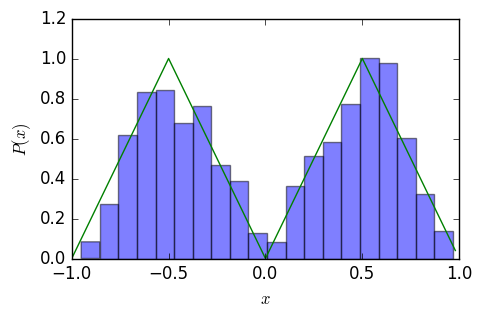
\includegraphics[valign=m,width=1.3in]{{plots/doublepeak1_0.1}.png}
		& 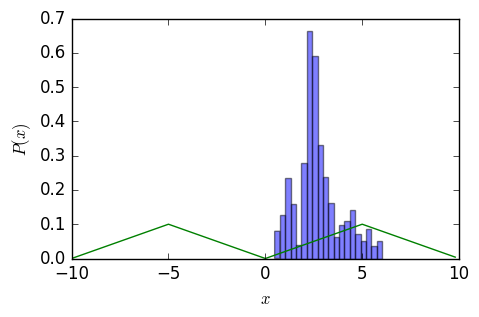
\includegraphics[valign=m,width=1.3in]{{plots/doublepeak10_0.1}.png}
		& 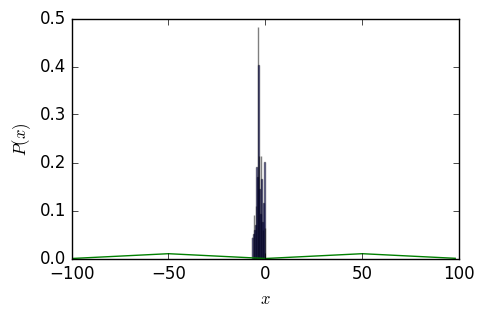
\includegraphics[valign=m,width=1.3in]{{plots/doublepeak100_0.1}.png}
		\\
		$\sigma=1$
		& 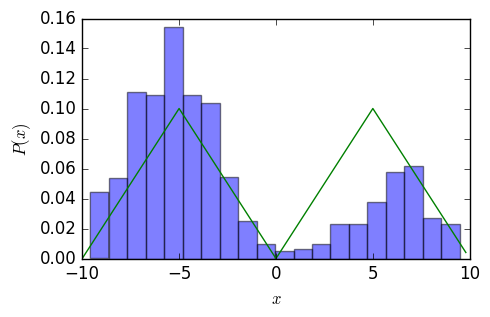
\includegraphics[valign=m,width=1.3in]{{plots/doublepeak10_1}.png}
		& 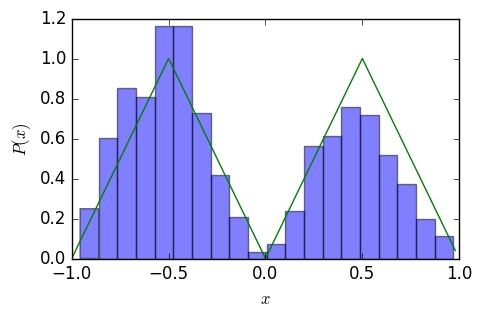
\includegraphics[valign=m,width=1.3in]{{plots/doublepeak1_1}.png}
		& 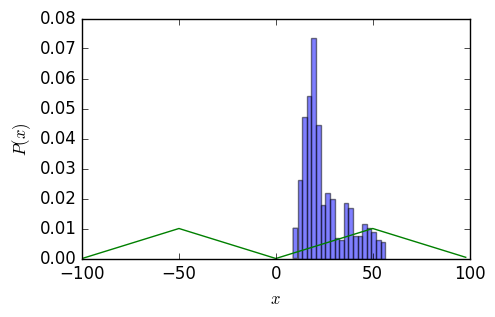
\includegraphics[valign=m,width=1.3in]{{plots/doublepeak100_1}.png}
		\\
		$\sigma=10$
		& 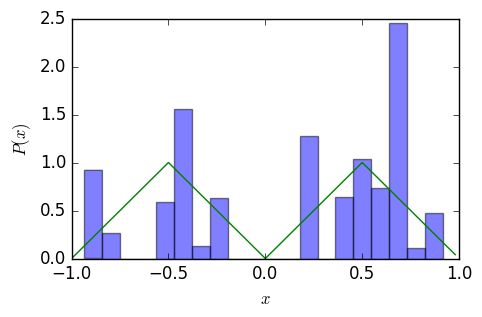
\includegraphics[valign=m,width=1.3in]{{plots/doublepeak1_10}.png}
		& 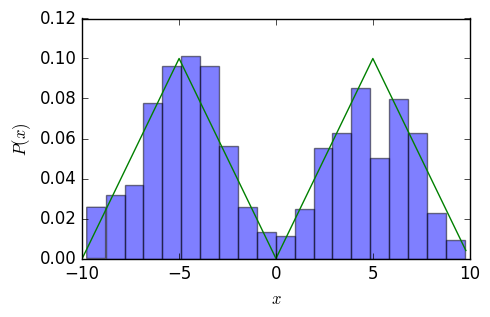
\includegraphics[valign=m,width=1.3in]{{plots/doublepeak10_10}.png}
		& 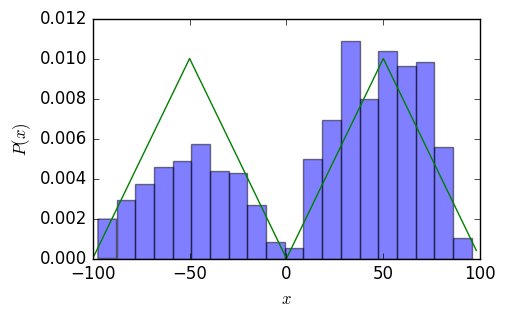
\includegraphics[valign=m,width=1.3in]{{plots/doublepeak100_10}.png}
		\\
		Adaptive
		& 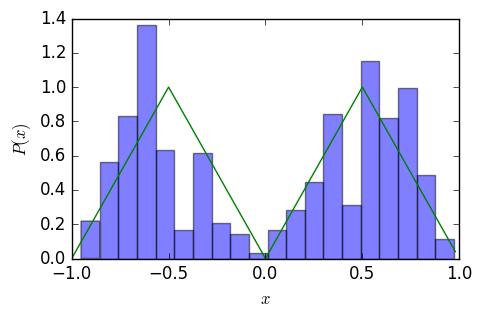
\includegraphics[valign=m,width=1.3in]{{plots/doublepeak1_adaptive}.png}
		& 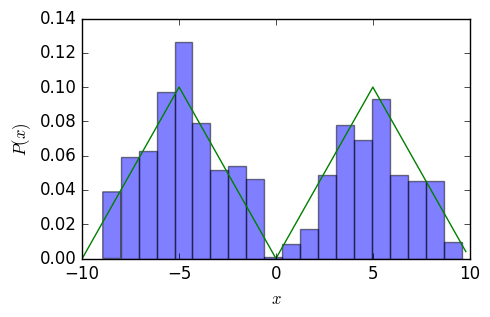
\includegraphics[valign=m,width=1.3in]{{plots/doublepeak10_adaptive}.png}
		& 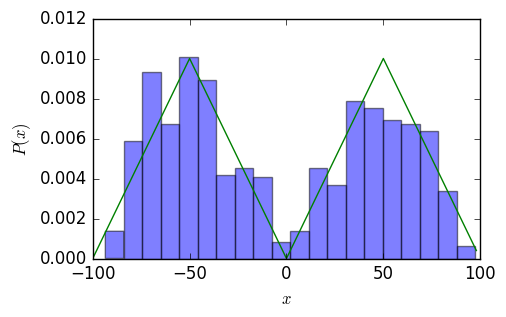
\includegraphics[valign=m,width=1.3in]{{plots/doublepeak100_adaptive}.png}
	\end{tabular}
	\caption{5000 samples (Burn-in 1000) of $p(x)=\max(\min(|x|,l-|x|),0)$}
	\label{fig:peaks}
\end{figure}

For this function, MH with a fixed proposal distribution explores the space well when $\sigma$ is tuned to the appropriate value. However, for all of the values of $\sigma$ in \cref{fig:peaks}, there are some values of $l$ for which MH does not approximate the distribution well. Either MH does not explore the entire space for larger $l$ or MH stays too long on the same sample for smaller $l$.

The adaptive variant does not suffer from these pitfalls and can reasonably fit the target distribution in all three cases.

\subsection{Rectangle Approximation to Images}

\begin{figure}[h!]
	\centering
	\begin{tabular}{lccc}
		Step & Nonadaptive ($\sigma=0.25\Sigma$) & Nonadaptive ($\sigma=0.05\Sigma$) & Adaptive \\[1em]
		500
		& \includegraphics[valign=m,width=1in]{generated/beach_25_500.png}
		& \includegraphics[valign=m,width=1in]{generated/beach_05_500.png}
		& \includegraphics[valign=m,width=1in]{generated/beach_adaptive_500.png}
		\\[4em]
		1000
		& \includegraphics[valign=m,width=1in]{generated/beach_25_1000.png}
		& \includegraphics[valign=m,width=1in]{generated/beach_05_1000.png}
		& \includegraphics[valign=m,width=1in]{generated/beach_adaptive_1000.png}
		\\[4em]
		2000
		& \includegraphics[valign=m,width=1in]{generated/beach_25_2000.png}
		& \includegraphics[valign=m,width=1in]{generated/beach_05_2000.png}
		& \includegraphics[valign=m,width=1in]{generated/beach_adaptive_2000.png}
		\\[4em]
		3000
		& \includegraphics[valign=m,width=1in]{generated/beach_25_3000.png}
		& \includegraphics[valign=m,width=1in]{generated/beach_05_3000.png}
		& \includegraphics[valign=m,width=1in]{generated/beach_adaptive_3000.png}
		\\[4em]
		4000
		& \includegraphics[valign=m,width=1in]{generated/beach_25_4000.png}
		& \includegraphics[valign=m,width=1in]{generated/beach_05_4000.png}
		& \includegraphics[valign=m,width=1in]{generated/beach_adaptive_4000.png}
		\\[4em]
		5000
		& \includegraphics[valign=m,width=1in]{generated/beach_25_5000.png}
		& \includegraphics[valign=m,width=1in]{generated/beach_05_5000.png}
		& \includegraphics[valign=m,width=1in]{generated/beach_adaptive_5000.png}
		\\[4em]
		Target
		&& 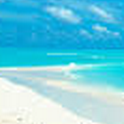
\includegraphics[valign=m,width=1in]{images/beach.png}
	\end{tabular}
	\caption{Progression using adaptive and nonadaptive MH}
	\label{fig:steps}
\end{figure}

In an application to computer vision, MCMC algorithms can be used to estimate the latent structure of an image. Goodman et al.\ \cite{dippl} use MH to infer a latent structure of colored rectangles which approximate an image. Among other things, similar techniques could be used to concisely represent the gist of an image in a thumbnail. I replicate the same and show that an adaptive MH can find a good approximation faster.

First, let's define the problem. Given an image, the target distribution encodes rectangles of random sizes, orientations, colors, and opacities. The negative log likelihood of a sample is the $\ell_1$ norm of the difference between the observed image and the image corresponding to overlaying the set of rectangles. The transition distribution is a Guassian with covariance matrix $\alpha\Sigma$, where $\Sigma$ encodes the full range of each of the parameters for a rectangle in the latent space.

Finally, both the nonadaptive and adaptive MH had better results when the proposal distribution picked a random rectangle to resample rather than resample all rectangles.

This comparison uses 8 rounded rectangles and a burn-in of 1000 samples. Empirically, the acceptance rate of 0.234 is reached when $\alpha\approx0.05$ for images. I show results for a fixed $\alpha=0.05$, fixed $\alpha=0.25$, and the adaptive MH.

\cref{fig:steps} demonstrates the progression of the adaptive and nonadaptive versions of MH. The adaptive version resembles the target image about as good as the $\sigma=0.05\Sigma$ fixed MH, and better than the $\sigma=0.25\Sigma$ fixed MH.

Additionally, there are a sample inferences on a number of target images in \cref{fig:output}. The adaptive MH yields good results as quickly as the best nonadaptive MH and does not require tuning of hyperparameters.

\begin{figure}[h]
	\centering
	\begin{tabular}{cccc}
		Nonadaptive ($\sigma=0.25\Sigma$) & Nonadaptive ($\sigma=0.05\Sigma$) & Adaptive & Target \\[1em]
		\includegraphics[valign=m,width=1in]{generated/beach_25_2000.png}
		& \includegraphics[valign=m,width=1in]{generated/beach_05_2000.png}
		& \includegraphics[valign=m,width=1in]{generated/beach_adaptive_2000.png}
		& 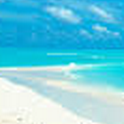
\includegraphics[valign=m,width=1in]{images/beach.png}
		\\[4em]
		\includegraphics[valign=m,width=1in]{generated/rectangles_25_2000.png}
		& \includegraphics[valign=m,width=1in]{generated/rectangles_05_2000.png}
		& \includegraphics[valign=m,width=1in]{generated/rectangles_adaptive_2000.png}
		& 
\includegraphics[valign=m,width=1in]{images/rectangles.png}
		\\[4em]
		\includegraphics[valign=m,width=1in]{generated/blue_25_2000.png}
		& \includegraphics[valign=m,width=1in]{generated/blue_05_2000.png}
		& \includegraphics[valign=m,width=1in]{generated/blue_adaptive_2000.png}
		& 
\includegraphics[valign=m,width=1in]{images/blue.png}
		\\[4em]
		\includegraphics[valign=m,width=1in]{generated/starry_25_2000.png}
		& \includegraphics[valign=m,width=1in]{generated/starry_05_2000.png}
		& \includegraphics[valign=m,width=1in]{generated/starry_adaptive_2000.png}
		& 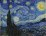
\includegraphics[valign=m,width=1in]{images/starry.jpg}
		\\[4em]
		\includegraphics[valign=m,width=1in]{generated/sunday_25_2000.png}
		& \includegraphics[valign=m,width=1in]{generated/sunday_05_2000.png}
		& \includegraphics[valign=m,width=1in]{generated/sunday_adaptive_2000.png}
		& \includegraphics[valign=m,width=1in]{images/sunday.jpg}
	\end{tabular}
	\caption{Results of adaptive and nonadaptive MH after 2000 steps}
	\label{fig:output}
\end{figure}

\section{Conclusion}

Adaptive MCMC is feasible and yields good results without the need to tune hyperparameters. Though adaptation needs to be tapered in order to keep asymptotic convergence guarantees valid, an adaptive MH can find a quickly-converging Markov chain without the need for fine tuning.

Adaptive MCMC has a wide variety of applications. I have demonstrated its use in computer vision for inferring latent parameters from a set of observations.

\nocite{*}
\bibliographystyle{acm}
\bibliography{bibliography}

\end{document}
